%! TEX program = pdflatex
%% Mauricio Caceres Bravo <mauricio.caceres.bravo@gmail.com>

%----------------------------------------------------------------------
\documentclass{article}

\usepackage[summary]{brownpreamble}
\usepackage{etoc}
\setcounter{tocdepth}{3}

\renewcommand{\subsectionmark}[1]{\markboth{#1}{}}
\renewcommand\sectiontype{Lecture \thesection:\ }
\lhead{\color{light-gray} \itshape Math Camp Aug 19, 2021 -- Lecture \thesection}
\rhead{\color{light-gray} \itshape \thesubsection. \leftmark}
\setcounter{section}{3}
% \renewcommand\SetHideLevel{1pt}

%----------------------------------------------------------------------
\begin{document}
\displayoptions

% ---------------------------------------------------------------------
\section{Differentiation, IFT, Unconstrained Optimization}
\label{sec:differentiation_ift_unconstrained_optimization}

\localtableofcontents

% ---------------------------------------------------------------------
\subsection{Differentiation}
\label{sub:differentiation}

\begin{definition}
  Let $I \in \mathbb{R}$ be an open interval; a function $f: I \to \mathbb{R}$ is \keyword{differentiable} at $a \in I$ if
  \[
    \lim_{x \to a} \dfrac{f(x) - f(a)}{x - a} = L
  \]

  for some $L$ (that is, the limit exists). We write $f^\prime(a) = L$ or $\dfrac{df}{dx}(a) = L$. If $f$ is  differentiable $\forall a \in I$ then we say $f$ is differentiable in $I$.
\end{definition}

Intuitively, differentiation yields the slope of a function at a point:
\begin{figure}[H]
  \centering
  \begin{tikzpicture}
    \begin{axis}[name=plot1
      %,title=
      ,width=15cm
      ,height=9cm
      ,ymin=1
      ,ymax=4.5
      ,xmin=0
      ,xmax=4.5
      ,domain=0:4
      %,ylabel=$y$
      %,xlabel=$x$
    ]
    \addplot [smooth] {4 * x - x^2};
    \addplot [only marks, mark=*] coordinates {(2, 4)};
    \addplot [only marks, mark=*, mark size=1pt] coordinates {
      (1,    3)
      (1.5,  3.75)
      (1.75, 3.9375)
    };
    \addplot [only marks, mark=*, mark size=1pt] coordinates {
      (3,    3)
      (2.5,  3.75)
      (2.25, 3.9375)
    };
    \addplot [smooth, domain=0.55:3.45] {4}
      node[above] at (axis cs:3.15, 4) {$f^\prime(a)$};

    % lim x -> a-
    \draw [->, >=latex] (axis cs:1.1, 1.125) -- (axis cs:1.5, 1.125);
    \draw [->, >=latex] (axis cs:1.5, 1.125) -- (axis cs:1.75,1.125);
    \draw [->, >=latex] (axis cs:1.75,1.125) -- (axis cs:1.9, 1.125);
    \node[above] at (axis cs:1.0, 1) {$x$};
    \node[above] at (axis cs:2.0, 1) {$a$};
    \addplot [smooth, dashed, domain=0.50:2] {4 + 1.0  * (x - 2)};
    \addplot [smooth, dashed, domain=0.75:2] {4 + 0.5  * (x - 2)};
    \addplot [smooth, dashed, domain=1.00:2] {4 + 0.25 * (x - 2)};

    % lim x -> a+
    \draw [->, >=latex] (axis cs:2.9, 1.125) -- (axis cs:2.5, 1.125);
    \draw [->, >=latex] (axis cs:2.5, 1.125) -- (axis cs:2.25,1.125);
    \draw [->, >=latex] (axis cs:2.25,1.125) -- (axis cs:2.1, 1.125);
    \node[above] at (axis cs:3.0, 1) {$x$};
    \addplot [smooth, dashed, domain=2:3.50] {4 - 1.0  * (x - 2)};
    \addplot [smooth, dashed, domain=2:3.25] {4 - 0.5  * (x - 2)};
    \addplot [smooth, dashed, domain=2:3.00] {4 - 0.25 * (x - 2)};

    \end{axis}
  \end{tikzpicture}
  \caption{Graphical representation of a derivative}
  \label{fig:graphical_representation_of_a_derivative}
\end{figure}

\begin{theorem}
  If $f: I \to \mathbb{R}$ is differentiable at $a \in I$ then $f$ is also continuous at $a$.
\end{theorem}

\begin{proof}
  We want to show that $\forall \varepsilon > 0 ~~ \exists \delta > 0$ s.t.
  \[
    |x - a| < \delta \implies |f(x) - f(a)| < \varepsilon
  \]

  Since $f$ is differentiable, we know that for any such $\varepsilon$, we can find some $\widetilde{\delta} > 0$ s.t.
  \[
    \dfrac{|f(x) - f(a)|}{\widetilde{\delta}}
    < \dfrac{|f(x) - f(a)|}{|x - a|}
    = \Fabs{\dfrac{f(x) - f(a)}{x - a} - L + L}
    \le \Fabs{\dfrac{f(x) - f(a)}{x - a} - L} + |L|
    < \varepsilon + |L|
  \]

  for some $L$. That is, we know the derivative exists and it is equal to some $L$, so by the definition of a limit, we can find $\widetilde{\delta} > 0$ s.t.
  \[
    |x - a| < \widetilde{\delta} \implies \Fabs{\dfrac{f(x) - f(a)}{x - a} - L} < \varepsilon
  \]

  Hence whenever $|x - a| < \widetilde{\delta}$ we get
  \[
    |f(x) - f(a)| < \left(\varepsilon + |L|\right) \widetilde{\delta}
  \]

  If we can find $\delta \le \widetilde{\delta}$ s.t. $\left(\varepsilon + |L|\right)\delta < \varepsilon$ then we'd be done. If $\widetilde{\delta} < 1$, then take $\delta = \widetilde{\delta} \cdot \dfrac{\varepsilon}{\varepsilon + |L|} \le \widetilde{\delta}$ (since $|L| \ge 0$, we multiply $\widetilde{\delta}$ by something $< 1$). Then we have
  \[
    |x - a| < \delta \le \widetilde{\delta}
    \implies
    |f(x) - f(a)|
    <
    \left(\varepsilon + |L|\right) \dfrac{\varepsilon}{\varepsilon + |L|} \widetilde{\delta}
    = \varepsilon \widetilde{\delta}
    < \varepsilon
  \]

  where the last inequality holds if $\widetilde{\delta} < 1$. If $\delta \ge 1$, then set $\delta = \dfrac{\varepsilon}{\varepsilon + |L|} \le 1 \le \delta$ and we get
  \[
    |x - a| < \delta \le \widetilde{\delta}
    \implies
    |f(x) - f(a)|
    <
    \left(\varepsilon + |L|\right) \dfrac{\varepsilon}{\varepsilon + |L|}
    = \varepsilon
  \]
\end{proof}

\begin{theorem}
  Let $f: I \to \mathbb{R}$ and $g: I \to \mathbb{R}$ be differentiable.
  \begin{itemize}[label=$\bullet$]
    \item $\dfrac{d}{dx} [c f(x)] = c f^\prime(x)$.
    \item $\dfrac{d}{dx} [f(x) + g(x)] = f^\prime(x) + g^\prime(x)$.
    \item \keyword{Product rule}: $\dfrac{d}{dx} f(x) g(x) = f^\prime(x) g(x) + f(x) g^\prime(x)$.
    \item \keyword{Power rule}: $\dfrac{d}{dx} x^k = k x^{k - 1}$.
    \item \keyword{Chain rule}: $(f \circ g)(x) = f(g(x)) = f^\prime(g(x)) g^\prime(x)$.
    \item \keyword{Quotient rule}: $\dfrac{f(x)}{g(x)} = \dfrac{f^\prime(x) g(x) - f(x) g^\prime(x)}{g(x)^2}$.
  \end{itemize}
\end{theorem}

Some useful special results:
\begin{align*}
  \dfrac{d}{dx} e^x & = e^x  \\
  \dfrac{d}{dx} \log(x) & = \dfrac{1}{x} \\
  \dfrac{d}{dx} \sin(x) & = \cos(x) \\
  \dfrac{d}{dx} \cos(x) & = -\sin(x)
\end{align*}

\begin{definition}
  A function $f: I \to \mathbb{R}$ is \keyword{continuously differentiable} if $f^\prime$ is continuous.
\end{definition}

\begin{example}
  $f(x) = x^2$ is continuously differentiable since $f^\prime(x) = 2x$ is continuous. However,
  \begin{align*}
    f(x) = \begin{cases}
      x^2 \sin(x) & x \ne 0 \\
      0 & x = 0
    \end{cases}
  \end{align*}

  is \textit{not} continuously differentiable. In particular, for $x \ne 0$,
  \begin{align*}
    f^\prime(x)
    =
    2 x \cos(1/x) - x^2 \dfrac{1}{x^2} \cos(1/x)
    =
    2 x \cos(1/x) - \cos(1/x)
  \end{align*}

  and for $x = 0$ the derivative is $0$:
  \begin{align*}
    \lim_{x \to 0}
    \dfrac{f(x) - f(0)}{x - 0}
    =
    \lim_{x \to 0}
    \dfrac{x^2 \sin(1/x)}{x}
    =
    \lim_{x \to 0}
    x \sin(1/x)
  \end{align*}

  With $\sin(1/x)$ bounded, $x \to 0 \implies x \sin(x) \to 0$. However, the derivative itself is not continuous  at $0$. Note that while $2x \cos(1/x) \xrightarrow{x \to 0} 0$, $- \cos(1/x)$ does not have a limit, so the derivative does not have a limit as $x \to 0$ either, meaning it cannot be continuous.
\end{example}

\begin{theorem}[L'H\^opital's rule.]\label{thm:lecture4_lhopital}
  Take $f, g: [a, b] \to \mathbb{R}$ be continuous functions on $[a, b]$ and differentiable on $(a, b)$ with $f(x), g(x) \ne 0$ for all $x \in (a, b)$. Further, let
  \[
    \lim_{x \to b} \dfrac{f^\prime(x)}{g^\prime(x)} = L
  \]

  and $g(b) = f(b) = 0$ or $\lim_{x \to b} g(b) = \lim_{x \to b} f(b) = 0$. Then
  \[
    \lim_{x \to b} \dfrac{f(x)}{g(x)} = L
  \]
\end{theorem}

\begin{theorem}[Taylor's theorem]
  Let $n \in \mathbb{N}$ and $f: [a, b] \to \mathbb{R}$ be continuously differentiable $n + 1$ times on $(a, b)$. Then for all $\widetilde{x}, x \in (a, b)$ there is some $c \in (\widetilde{x}, x)$ s.t.
  \[
    f(x)
    = \sum^{n}_{k = 0} \dfrac{f^{(k)}(\widetilde{x})}{k!} (x - \widetilde{x})^k
    + \dfrac{f^{(n + 1)}(c)}{(n + 1)!} (x - \widetilde{x})^{n + 1}
  \]

  The first term is called the \keyword{$n$th order Taylor expansion} of $f$ around $\widetilde{x}$.
\end{theorem}

\begin{example}
  \begin{itemize}[label=$\bullet$]
    \item The Taylor expansion of any polynomial is the polynomial itself. Consider
      \[
        f(x) = x^2 + 3x
      \]

      \begin{align*}
        f(x)
        & =
        \dfrac{f(1)}{0!} (x - 1)^0
        +
        \dfrac{f^\prime(1)}{1!} (x - 1)^1
        +
        \dfrac{f^{\prime\prime}(c)}{2!} (x - 1)^2
        \\
        & =
        4
        +
        5 (x - 1)
        +
        \dfrac{2}{2} (x - 1)^2
        \\
        & =
        4 + 5x - 5 + x^2 - 2x + 1
        =
        x^2 + 3x
      \end{align*}

      However, for lower-order Taylor expansions the theorem still applies. Visually:
      \begin{figure}[H]
        \centering
        \caption{Visualizing Taylor's Theorem}
        \label{fig:visualizing_taylor_s_theorem}
        \begin{tikzpicture}
          \begin{axis}[name=plot1
            ,title={Given $x = 5$ Recover Exact Value}
            ,width=9cm
            ,height=8cm
            ,ymin=0
            ,ymax=6
            ,xmin=0
            ,xmax=1.5
            ,domain=0:1.5
            ,ylabel={$f(x) = x^2 + 3x$}
            ,xlabel=$x$
            ,clip=false
          ]
          \addplot [smooth,domain=0:1.25] {x^2 + 3 * x};
          \addplot [smooth,domain=0.1:1.15] {4 + (2 * (3/4) + 3) * (x - 1)};
          \draw [dashed] (axis cs:0.5, 1.75) -- (axis cs:0.5, 0);
            \node[below] at (axis cs:0.5, 0) {$x = 0.5$};
          \draw [->, >=latex] (axis cs:0.5, 3.5) -- (axis cs:0.5, 1.95);
            \node[above] at (axis cs:0.5, 3.5) {$c = 0.75 \in (0.5, 1)$};
          \addplot [only marks, mark=*] coordinates {(0.5, 1.75)};
          \end{axis}

          \begin{axis}[name=plot2
            ,title={Approximate the function around $x = 1$}
            ,at={($(plot1.east) + (0.5cm, 0)$)}
            ,anchor=west
            ,width=9cm
            ,height=8cm
            ,ymin=0
            ,ymax=7
            ,xmin=0
            ,xmax=1.75
            ,domain=0:1.75
            ,ylabel={$f(x) = x^2 + 3x$}
            ,xlabel=$x$
            ,clip=false
          ]
          \addplot [smooth,domain=0:1.5] {x^2 + 3 * x};
          \addplot [smooth,domain=0.15:1.5] {4 + 5 * (x - 1)};
          \draw [dashed] (axis cs:1, 4) -- (axis cs:1, 0);
            \node[below] at (axis cs:1, 0) {$x = 1$};
          \addplot [only marks, mark=*] coordinates {(1, 4)};
          \draw [->, >=latex] (axis cs:1.35, 4.75) -- (axis cs:1.35, 5.65);
            \node[below] at (axis cs:1.35, 4.75) {$5x - 1$};
          \end{axis}
        \end{tikzpicture}
      \end{figure}

      The left and right figures correspond to:
      \begin{align*}
        f(x)
        & = \dfrac{f(1)}{0!} (x - 1)^0 + \dfrac{f^\prime(c)}{1!} (x - 1)^1
        \\
        & = 4 + (2c + 3) (x - 1)
        \\
        f(x)
        & \approx \dfrac{f(1)}{0!} (x - 1)^0 + \dfrac{f^\prime(1)}{1!} (x - 1)^1
        \\
        & = 4 + 5 (x - 1)
      \end{align*}

      We can see on the left that there is indeed some number $c$ s.t. Taylor's theorem holds. For our sample value of $x = 0.5$ we find $c = 0.75 \in (0.5, 1)$. On the right figure, on the other hand, we plot the \textit{approximation}. In this case, the function and the approximation are exactly equal at $1$, since the approximation at that point simplifies to $f(1)$. We can also see that around $x = 1$ the approximation is fairly good! However, farther away the error increases, as we would expect.

    \item One common Taylor approximation is for the logarithm. In particular, the first order Taylor expansion around  $1$:
      \begin{align*}
        \log(x) \approx \log(1) + \dfrac{1}{1} (x - 1) = x - 1
      \end{align*}

      Another version of this approximation is for $\log(1 + x)$ around $0$:
      \begin{align*}
        \log(1 + x) \approx \log(1) + \dfrac{1}{1 + 0} (x - 0) = x
      \end{align*}

      Take the relation:
      \begin{align*}
        \log Y = \alpha \log K + (1 - \alpha) \log L
      \end{align*}

      Using the approximation above, we can say that if $K$ increases by $10\%$, then $Y$ increases by $\alpha \log (1.1) \approx \alpha \cdot 0.1$, that is, $10\alpha \%$.
  \end{itemize}

  This second approximation is often used when dealing with percentage changes. You will hear the term \keyword{log-linearization}  thrown around, and this is what that's in reference to: Logarithms can be approximated as a percentage for small values.
\end{example}

\subsubsection{Partial Derivatives}
\label{ssub:partial_derivatives}

\begin{definition}
  Let $f: S \subseteq \mathbb{R}^N \to \mathbb{R}^M$, $e = (e_1, \ldots, e_N)$ a standard basis of $\mathbb{R}^N$, $u = (u_1, \ldots, u_M)$ a standard basis for $\mathbb{R}^M$. $\forall x \in S, f(x) \in \mathbb{R}^M$, $f(x)$ is a linear combination of $u$ and some set of functions $\set{f_1, \ldots, f_M}$ s.t. $f_i: S \to \mathbb{R}$ with
  \[
    f(x) = \sum^{M}_{i = 1} f_i(x) u_i
  \]
\end{definition}

\begin{definition}
  The \keyword{partial derivative} of a function $f: S \subseteq \mathbb{R}^N \to \mathbb{R}^M$ at $x \in S$ is
  \[
    \dfrac{\partial}{\partial x_j} f_i(x) = \lim_{t \to 0} \dfrac{f_i(x + t \cdot e_j) - f_i(x)}{t}
  \]

  for $i = 1, \ldots, M$ and $j = 1, \ldots, N$.
\end{definition}

% \begin{theorem}
%   Let $f: S \subseteq \mathbb{R}^N \to \mathbb{R}^M$ be differentiable at $x \in S$. Then all partial derivatives exist and
%   \[
%     f^\prime(x) \cdot e_j = \sum^{M}_{i = 1} u_i \cdot \dfrac{\partial}{\partial x_j} f_i(x)
%   \]
% \end{theorem}
%
% \begin{tacomment}{0}
%   I object to this theorem because we haven't defined what it means for a a function $f: S \subseteq \mathbb{R}^N \to \mathbb{R}^M$ to be differentiable! We have defined that a partial derivative is.
% \end{tacomment}

Note that partial derivatives needn't imply anything about the behavior of the function overall. Take, for instance, $f: \mathbb{R}^2 \to \mathbb{R}$ with
\[
  f(x, y) =
  \begin{cases}
    \dfrac{xy^2}{x^2 + y^4} & (x, y) \ne (0, 0) \\
    0 & (x, y) = (0, 0)
  \end{cases}
\]

The partial derivatives at $0$ are all $0$ (crucially, we take the limits one dimension at a time, so it's not that $(x, y) \to (0, 0)$, but rather $x \to 0$ and then $y \to 0$. Now take any $y_m \to 0$ and $x_m = y_m^2$ s.t. $y_m \ne 0$ for all $n$.
\[
  \lim_{n \to \infty} f(x_m, y_m) = \dfrac{1}{2} \ne 0
\]

which means the function is not even continuous at $0$.
% , and hence it cannot be differentiable.\footnote{Again, we haven't defined differentiability in this context.}

\begin{theorem}[Schwarz's Theorem]
  Let $f: S \subseteq \mathbb{R}^N \to \mathbb{R}$; then
  \[
    \dfrac{\partial}{\partial x_i} \dfrac{\partial}{\partial x_j} f(x)
    =
    \dfrac{\partial}{\partial x_j} \dfrac{\partial}{\partial x_i} f(x)
  \]

  if all the partial derivatives exist. That is, mixed partial derivatives are symmetric (if they exist).
\end{theorem}

\begin{definition}
  Let $f: S \subseteq \mathbb{R}^N \to \mathbb{R}^M$ and $x \in S$; $(Df)(x)$ is a $N \times M$ matrix with $i, j$ entry equal to $\dfrac{\partial}{\partial x_i} f_j(x)$.
\end{definition}

\begin{definition}
  The \keyword{gradient} of $f: S \subseteq \mathbb{R}^N \to \mathbb{R}$ at $x \in S$ is
  \[
    (\nabla f)(x) = \left[\begin{matrix}
      \dfrac{\partial}{\partial x_1} f(x) \\
      \vdots \\
      \dfrac{\partial}{\partial x_N} f(x) \\
    \end{matrix}\right]
  \]

  The gradient can also be denoted as $(Df)(x)$.
\end{definition}

\begin{definition}
  The \keyword{Hessian} of $f: S \subseteq \mathbb{R}^N \to \mathbb{R}$ at $x \in S$ is
  \[
    (D^2 f)(x) = \left[\begin{matrix}
      \dfrac{\partial^2}{\partial x_1^2} f(x) & \cdots & \dfrac{\partial^2}{\partial x_N \partial x_1} f(x) \\
      \vdots & \ddots & \vdots \\
      \dfrac{\partial}{\partial x_1 \partial x_N} f(x) & \cdots & \dfrac{\partial^2}{\partial x_N^2} f(x) \\
    \end{matrix}\right]
  \]

  Where $D^2$ denotes the application of the $D$ operator twice.
\end{definition}

\subsubsection{Mean Value Theorem (MVT)}
\label{ssub:mean_value_theorem_mvt_}

\begin{theorem}[Mean Value Theorem (MVT)]\label{thm:lecture4_mvt}
  Let $f: [a, b] \to \mathbb{R}$ be a continuous function on the closed interval $[a, b]$ and differentiable on the open interval $(a, b)$. Then $\exists c \in (a, b)$ s.t.
  \[
    f^\prime(c) = \dfrac{f(b) - f(a)}{b - a}
  \]
\end{theorem}

We will prove an equivalent, albeit perhaps conceptually easier, version of this:
\begin{theorem}[Rolle's Theorem]\label{thm:lecture4_rolles_theorem}
  Let $g: [a, b] \to \mathbb{R}$ be continuous on $[a, b]$ and differentiable on $(a, b)$ with $g(a) = g(b)$. Then $\exists c \in (a, b)$ s.t.
  \[
    f^\prime(c) = 0
  \]
\end{theorem}

\begin{figure}[!ht]
  \centering
  \begin{tikzpicture}
    \begin{axis}[name=plot1
      ,title={Mean Value Theorem}
      ,width=9cm
      ,height=8cm
      ,ymin=0
      ,ymax=3
      ,xmin=0
      ,xmax=2
      ,domain=0.25:1.75
      %,ylabel=$y$
      %,xlabel=$x$
    ]
    \addplot [smooth] {1 + (x - 0.5)^2}
      node[above] at (axis cs:0.25,   1.1625) {$f(a)$}
      node[above] at (axis cs:1.75,   2.6125) {$f(b)$}
      node[below] at (axis cs:1.0167, 1.167)  {$f(c)$};
    \addplot [smooth, dashed] {0.2167 + 1.033 * x}
      node[below] at (axis cs:1.75, 1.9) {$f^\prime(c)$};
    \addplot [only marks, mark=*] coordinates {
      (0.25,   1.0625)
      (1.75,   2.6125)
      (1.0167, 1.267)
    };
    \draw [dashed]
      (axis cs:0.25, 1.0625) --
      (axis cs:1.75, 2.6125);
    \end{axis}

    \begin{axis}[name=plot2
      ,title={Rolle's Theorem}
      ,at={($(plot1.east) + (0.5cm, 0)$)}
      ,anchor=west
      ,width=9cm
      ,height=8cm
      ,ymin=0
      ,ymax=4
      ,xmin=0
      ,xmax=4
      ,domain=0.25:3.75
      %,ylabel=$y$
      %,xlabel=$x$
    ]
    \addplot [smooth] {0.25 + (x - 2)^2}
      node[above] at (axis cs:0.25,   3.3125) {$f(a)$}
      node[above] at (axis cs:3.75,   3.3125) {$f(b)$}
      node[above] at (axis cs:2,      0.3)    {$f(c)$};
    \addplot [smooth, dashed] {0.25}
      node[below] at (axis cs:3.5, 0.6) {$f^\prime(c)$};
    \addplot [only marks, mark=*] coordinates {
      (0.25,   3.3125)
      (3.75,   3.3125)
      (2,      0.25)
    };
    \draw [dashed]
      (axis cs:0.25, 3.3125) --
      (axis cs:3.75, 3.3125);
    \end{axis}
  \end{tikzpicture}
  \caption{Graphical depiction of MVT}
  \label{fig:graphical_depiction_of_mvt}
\end{figure}

\begin{claim}
  \nameref{thm:lecture4_rolles_theorem} iff \nameref{thm:lecture4_mvt}.
\end{claim}

\begin{proof}
  The mean value theorem implies Rolle's theorem by definition. Simply note that by the MVT there is some $c$ s.t.
  \[
    f^\prime(c) = \dfrac{g(b) - g(a)}{b - a} = 0
  \]

  Now to show Rolle's theorem implies MVT, we only need a simple transformation:
  \[
    g(x) = \left(f(x) - f(a)\right) - \dfrac{f(b) - f(a)}{b - a} (x - a)
  \]

  Note that $g(a) = g(b) = 0$. Hence $\exists c$ s.t.
  \[
    g^\prime(c) = 0
  \]

  But we can see that
  \[
    g^\prime(c) = f^\prime(c) - \dfrac{f(b) - f(a)}{b - a} = 0
    \implies
    f^\prime(c) = \dfrac{f(b) - f(a)}{b - a}
  \]
\end{proof}

Now we show \nameref{thm:lecture4_rolles_theorem}.
\begin{proof}
    For Rolle's theorem we will use the extreme value theorem, and we know that $f$ is bounded and attains its $\sup$ and its $\inf$ in $[a, b]$. If the $\sup$ and the $\inf$ are \textit{both} at $\set{a, b}$, then because by assumption $f(a) = f(b) = 0$, $f(x) = 0$ everywhere on $[a, b]$. Take any $c \in (a, b)$, and
    \[
        f^\prime(c)
        = \lim_{y \to c} \dfrac{f(y) - f(c)}{y - c}
        = \lim_{y \to c} \dfrac{0}{y - c}
        = \lim_{y \to c} 0 = 0
    \]

    Suppose then that either the $\sup$ or the $\inf$ occur at at interior point $c \in (a, b)$. Take the $\sup$ (the case for the $\inf$ will be analogous). By assumption $f$ is differentiable, so $f^\prime(c)$ exists. That is, we know that
    \[
        f^\prime(c)
        = \lim_{y \to c} \dfrac{f(y) - f(c)}{y - c}
        = L
    \]

    Consider $y \to c^-$, that is $y$ approaching $c$ from the left. Since the $\sup$ is attained at $c$, $f(c) \ge f(y)$ for all $c > y$, which in turn gives
    \[
        \dfrac{f(y) - f(c)}{y - c} \ge 0
        \quad\quad
        \forall c > y
    \]

    Now take $y \to c^+$, that is $y$ approaching $c$ from the right. Again, since the $\sup$ is attained at $c$, $f(c) \ge f(y)$ for all $c < y$, which in turn gives
    \[
        \dfrac{f(y) - f(c)}{y - c} \le 0
        \quad\quad
        \forall c < y
    \]

    Which means that
    \[
        L_- = \lim_{y \to c^-} \dfrac{f(y) - f(c)}{y - c} \ge 0
    \]

    Suppose not, then $L_- < 0$. But for every $\varepsilon > 0$ there is some $\delta$ s.t.
    \[
        c^- - \delta < y < c^- < c^- + \delta
        \implies
        L_- - \varepsilon < \dfrac{f(y) - f(c)}{y - c} < L_- + \varepsilon
    \]

    Take $\varepsilon$ s.t. $L_- < - \varepsilon < 0$. Then for some $\delta > 0$, we get
    \[
        c^- - \delta < y < c^- < c^- + \delta
        \implies
        L_- - \varepsilon < \dfrac{f(y) - f(c)}{y - c} < L_- + \varepsilon < 0
    \]

    But we have established that $y < c$ gives $\dfrac{f(y) - f(c)}{y - c} \ge 0$, a contradiction. By that same logic, we can write
    \[
        L_+ = \lim_{y \to c^+} \dfrac{f(y) - f(c)}{y - c} \le 0
    \]

    Since $f^\prime(c)$ exists, it must be the case that
    \[
        f^\prime(c)
        = \lim_{y \to c^+} \dfrac{f(y) - f(c)}{y - c}
        = L_+
        = \lim_{y \to c^-} \dfrac{f(y) - f(c)}{y - c}
        = L_-
        = L
    \]

    Now we can see that $L_+ \le 0$, $L_- \ge 0$, and $L_+ = L_- = L$  gives that $L = 0$. The proof for the case when the $\inf$ is interior is completely analogous.
\end{proof}

\begin{corollary}
  If $f$ is continuous on $[a, b]$ and differentiable on $(a, b)$ and obtains a local minimum or maximum at $c$, then $f^\prime(c) = 0$.
\end{corollary}

\begin{corollary}
  If $f$ is continuous on $[a, b]$ and differentiable on $(a, b)$ and $f^\prime(x) > 0$ for every $x \in (a, b)$ then $f$ is increasing on $(a, b)$. Conversely, if $f^\prime(x) < 0$ for every $x \in (a, b)$ then $f$ is decreasing on $(a, b)$.
\end{corollary}

\begin{theorem}[Generalized MVT]
  Let $f, g: [a, b] \to \mathbb{R}$ be continuous functions on $[a, b]$ and differentiable on $(a, b)$. Then $\exists c \in (a, b)$ s.t.
  \[
    g^\prime(c) \left(f(b) - f(a)\right)
    =
    f^\prime(c) \left(g(b) - g(a)\right)
  \]
\end{theorem}

The MVT is a case where $g(x) = x$, the identity function.

% ---------------------------------------------------------------------
\subsection{Implicit Function Theorem (IFT)}
\label{sub:implicit_function_theorem_ift_}

\subsubsection{Motivation}
\label{ssub:motivation}

Consider a function $f(x, y) = 0$. How do we characterize a function relating $x$ to $y$? We can write that for $f: \mathbb{R}^2 \to \mathbb{R}$ continuously differentiable on an open set $O$ with $f(x, y) = 0$, there exists some function $h$ s.t.
\[
  f(x, h(x)) = 0
  \text{ and }
  \dfrac{dy}{dx} = -\dfrac{\partial f / \partial x}{\partial f / \partial y}
\]

One classic example is how to characterize the slope of a tangent line at a point $(x, y)$ of some circle of radius $r$ centered at $(0, 0)$. That is, $x^2 + y^2 = r^2$. We can write
\[
  f(x, y) = x^2 + y^2 - r^2 = 0
\]

So we know that for some $h(x)$, $f(x, h(x)) = 0$. Furthermore,
\[
  \dfrac{\partial f}{\partial x}
  = 2x
  \quad
  \dfrac{\partial f}{\partial y}
  = 2y
  \implies
  \dfrac{dy}{dx}
  = - \dfrac{x}{y}
\]

We will look at the general version of the theorem. We often work with a parameter space and a variable space, and we  want to express the variables in terms of the parameters (or with exogenous and endogenous variables, and we want to express the endogenous variables in terms of the exogenous variables). Take
\[
  (\theta_1, \ldots, \theta_N) = \theta \in \mathbb{R}^N
\]

to be the parameters (or exogenous) and
\[
  (x_1, \ldots, x_M) = x \in \mathbb{R}^M
\]

to be the variables (or endogenous). It's typically not common to have an explicit expression for the latter in terms of the former, but often we will encounter an implicit relation of the form
\[
  f(\theta, x) = 0
\]

For example, some system of equations
\begin{equation}
  \begin{array}{c}
    f_1(\theta, x) = 0 \\
    \vdots \\
    f_M(\theta, x) = 0
  \end{array}
  \nonumber
\end{equation}

The IFT gives a result we can apply to these types of problems.

\subsubsection{The IFT}
\label{ssub:the_ift}

\begin{theorem}[Implicit Function Theorem (IFT)]
  Take a function $f: \mathbb{R}^N \times \mathbb{R}^M \to \mathbb{R}^M$ that is continuously differentiable and fix a point $(\widetilde{\theta}, \widetilde{x}) \in \mathbb{R}^N \times \mathbb{R}^M$ s.t. $f(\widetilde{\theta}, \widetilde{x}) = 0$. If $D_x f(\widetilde{\theta}, \widetilde{x})$ is non-sigular (i.e. full-rank, or has a non-0 determinant) then for some open sets $A, B$ s.t. $\widetilde{\theta} \in A$, $\widetilde{x} \in B$, there exist a unique function $h: A \to B$ that is continuously differentiable in $A$ s.t.
  \[
    f(\theta, h(\theta)) = 0
  \]

  for all $\theta \in A$, and $h(\widetilde{\theta}) = \widetilde{x}$. Taking derivatives with respect to $\theta$, we further have
  \[
    D_\theta f(\theta, h(\theta)) + D_x f(\theta, h(\theta)) D_\theta h(\theta) = 0
  \]
  \[
    D_\theta h(\theta) = - \left[D_x f(\theta, h(\theta))\right]^{-1} D_\theta f(\theta, h(\theta))
  \]
\end{theorem}

\subsubsection{Example}
\label{ssub:example}

Take a simplified version of the IS-LM model
\begin{align*}
  Y   & = C + I + G   \\
  C   & = C(Y - T)    \\
  I   & = I(r)        \\
  M^S & = M^D(Y, r)
\end{align*}

with
\[
  0 < C^\prime(x) < 1
  \quad\quad
  I^\prime(r) < 0
  \quad\quad
  \dfrac{\partial M^D}{\partial Y} > 0
  \quad\quad
  \dfrac{\partial M^D}{\partial r} < 0
\]

National income must equal consumption plus investment (savings) plus government spending; consumption is some function of income minus taxes, the level of investment is determined by the interest rate, and money supply must equal money demand.  We have that
\begin{align*}
  Y - C(Y - T) - I(r) - G & = 0 \\
  M^S - M^D (Y, r)        & = 0
\end{align*}

which is the exact type of problem the IFT can help us solve. We have endogenous variables $x = (Y, r)$, national income and the interest rate, and exogenous variables $\theta = (M^S, G, T)$, money supply, government spending, and taxes. Hence
\begin{equation}
 \label{eq:is_lm_example}
  f(\theta, x)
  =
  \left[\begin{matrix}
    f_1(\theta, x) \\
    f_2(\theta, x)
  \end{matrix}\right]
  =
  \left[\begin{matrix}
    Y - C(Y - T) - I(r) - G \\
    M^S - M^D (Y, r)
  \end{matrix}\right]
  = 0
\end{equation}

Hence for some $h$, we can write
\begin{equation}
  \begin{array}{c}
    h(\theta)
    = \left[\begin{matrix}
      Y(M^S, G, T) \\
      r(M^S, G, T)
    \end{matrix}\right] \\[6pt]
    D_\theta f(\theta, h(\theta)) + D_x f(\theta, h(\theta)) D_\theta h(\theta) = 0
  \end{array}
  \nonumber
\end{equation}

We have that
\begin{align*}
  D_\theta f(\theta, h(\theta))
  & =
  \left[\begin{matrix}
      0
    & -1
    & C^\prime(Y(\cdot) - T) \\[6pt]
      1
    & 0
    & 0
  \end{matrix}\right] \\[6pt]
  D_x f(\theta, h(\theta))
  & =
  \left[\begin{matrix}
      \dfrac{\partial f_1}{\partial Y} = 1 - C^\prime(Y(\cdot) - T)
    & \dfrac{\partial f_1}{\partial r} = -I^\prime(r(\cdot)) \\[6pt]
      \dfrac{\partial f_2}{\partial Y} = -\dfrac{\partial M^D}{\partial Y}
    & \dfrac{\partial f_2}{\partial r} = -\dfrac{\partial M^D}{\partial r}
  \end{matrix}\right] \\[6pt]
  \left[D_x f(\theta, h(\theta))\right]^{-1}
  & =
  \dfrac{1}{D}
  \left[\begin{matrix}
      - \dfrac{\partial M^D}{\partial r}
    & I^\prime(r(\cdot)) \\[6pt]
      \dfrac{\partial M^D}{\partial Y}
    & 1 - C^\prime(Y(\cdot) - T)
  \end{matrix}\right] \\[6pt]
  D & =
  \underbrace{
   - \overbrace{\dfrac{\partial M^D}{\partial r}}^{< 0}
     \underbrace{\Bpar{1 - C^\prime(Y(\cdot) - T)}}_{> 0}
   }_{> 0}
  \underbrace{
   - \overbrace{I^\prime(r(\cdot))}^{< 0}
     \underbrace{\dfrac{\partial M^D}{\partial Y}}_{> 0}
   }_{> 0}
   \implies D > 0
\end{align*}

A non-zero determinant implies that the inverse exists. Hence we find that
\begin{align*}
  D_\theta h(\theta)
  & =
  \left[\begin{matrix}
      \dfrac{\partial Y}{\partial M^S}
    & \dfrac{\partial Y}{\partial G}
    & \dfrac{\partial Y}{\partial T} \\[6pt]
      \dfrac{\partial r}{\partial M^S}
    & \dfrac{\partial r}{\partial G}
    & \dfrac{\partial r}{\partial T}
  \end{matrix}\right]
  =
  - \dfrac{1}{D}
  \left[\begin{matrix}
        I^\prime(r(\cdot))
    &   \dfrac{\partial M^D}{\partial r}
    & - \dfrac{\partial M^D}{\partial r} C^\prime(Y(\cdot) - T)
    \\[6pt]
        1 - C^\prime(Y(\cdot) - T)
    & - \dfrac{\partial M^D}{\partial Y}
    &   \dfrac{\partial M^D}{\partial Y} C^\prime(Y(\cdot) - T)
    \\[6pt]
  \end{matrix}\right] \\
  & =
  - \dfrac{1}{D}
  \left[\begin{matrix}
      < 0
    & < 0
    & > 0 \\[6pt]
      > 0
    & < 0
    & > 0
  \end{matrix}\right]
  =
  \dfrac{1}{D}
  \left[\begin{matrix}
      > 0
    & > 0
    & < 0 \\[6pt]
      < 0
    & > 0
    & < 0
  \end{matrix}\right]
\end{align*}

Which means that for some $x = (Y, r), \theta = (M^S, G, T)$ that satisfies \Cref{eq:is_lm_example} there is some local neighborhood around $\theta$ where we can characterize the behavior of $(Y, r)$ with respect to each of the variables in $\theta$. In particular, income reacts positively to increases money supply or government spending but negatively to taxes, while the interest rate goes down with increases in the money supply or taxes but goes up with increases in government spending.

% ---------------------------------------------------------------------
\subsection{Unconstrained Optimization}
\label{sub:unconstrained_optimization}

\begin{definition}
  Let $f: A \to B$
  \begin{enumerate}
    \item $x \in A$ is a \keyword{local maximum} of $f$ if $\exists \varepsilon > 0$ s.t.
      \[
        y \in B_\varepsilon(x) \cap A \implies f(x) \ge f(y)
      \]

      The local maximum is \textbf{\textit{strict}} if the inequality is strict. (Note the intersection: For example, $f(x) = x$ has no local maximum on $\mathbb{R}$, but every point is a local maximum if we define the function over $x \in \mathbb{N}$.)

    \item The \keyword{local minimum} definition is analogous.

    \item $x \in A$ is a \keyword{global maximum} of $f$ if $\forall y \in A$, $f(x) \ge f(y)$. It is a strict global maximum if whenever $x \ne y$ we have $f(x) > f(y)$.

    \item The \keyword{global minimum} definition is analogous.
  \end{enumerate}
\end{definition}

\begin{figure}[!ht]
  \centering
  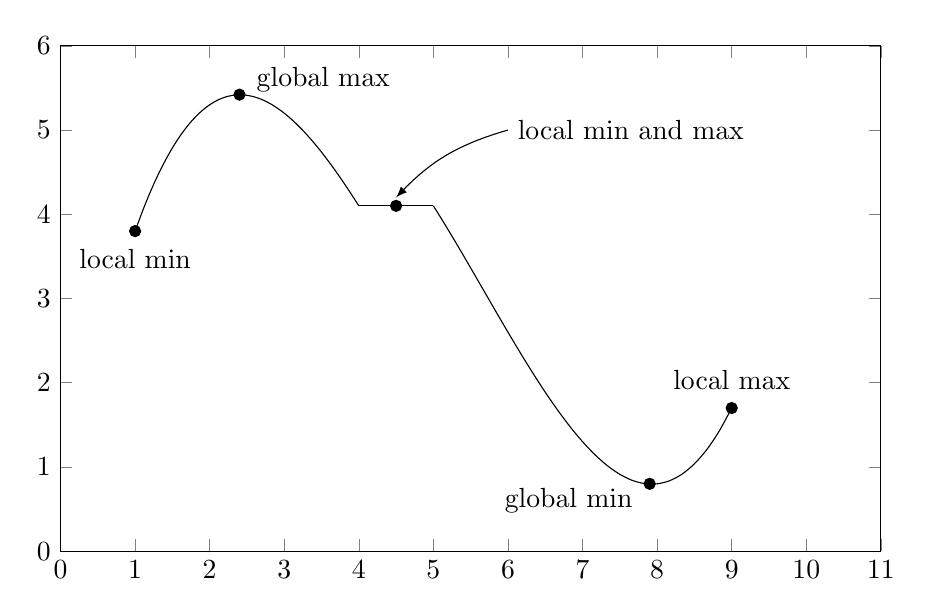
\begin{tikzpicture}
    \begin{axis}[name=plot1
      %,title=
      ,width=12cm
      ,height=8cm
      ,ymin=0
      ,ymax=6
      ,xmin=0
      ,xmax=11
      ,domain=1:9
      %,ylabel=$y$
      %,xlabel=$x$
    ]
    \addplot [smooth,domain=1:4] {0.1 * (x - 4)^3 - 0.2 * x^2 + 0.2 * x + 6.5};
    \addplot [smooth,domain=5:9] {0.1 * (x - 5)^3 - 0.2 * (x - 1)^2 + 0.2 * (x - 1) + 6.5};
    \draw [-] (axis cs:4, 4.1) -- (axis cs:5, 4.1) ;
    \addplot [only marks, mark=*] coordinates {
      (1, 3.8)
      (2.4, 5.42)
      (7.9, 0.8)
      (9, 1.7)
      (4.5, 4.1)
    };
    \node[below] at (axis cs:1,   3.7) {local min};
    \node[right] at (axis cs:2.5, 5.6) {global max};
    \node[left]  at (axis cs:7.8, 0.6) {global min};
    \node[above] at (axis cs:9,   1.8) {local max};
    \draw [->, >=latex]
      (axis cs:6, 5) to[bend right=15] (axis cs:4.5, 4.2)
      node[right] at (axis cs:6, 5) {local min and max};
    \end{axis}
  \end{tikzpicture}
  \caption{Examples of local and global maxima and minima}
  \label{fig:examples_of_local_and_global_maxima_and_minima}
\end{figure}

\begin{definition}
  The \keyword{$\argmax$} of a function $f$ is the set
  \[
    \argmax_{x \in A} f(x) = \Fset{x \in A: f(x) \ge f(y) ~~ \forall y \in A}
  \]

  The \keyword{$\argmin$} is analogously defined.
\end{definition}

\subsubsection{Linear Algebra Review}
\label{ssub:linear_algebra_review}

\begin{definition}
  A square $N \times N$ matrix $S$ with elements in $\mathbb{R}$ is \keyword{positive semidefinite} (PSD) if $\forall p \in \mathbb{R}^N$ we have
  \[
    p^T S p \ge 0
  \]

  and \keyword{positive definite} (PD) if the inequality is strict.
\end{definition}

\begin{definition}
  A square $N \times N$ matrix $S$ with elements in $\mathbb{R}$ is \keyword{negative semidefinite} (NSD) if $\forall p \in \mathbb{R}^N$ we have
  \[
    p^T S p \le 0
  \]

  and \keyword{negative definite} (ND) if the inequality is strict.
\end{definition}

\begin{definition}
  Let $S$ be a $N \times N$ matrix with elements in $\mathbb{R}$. If $\exists p_1, p_2 \in \mathbb{R}^N$ s.t.
  \[
    p_1^T S p_1 > 0
    \quad
    \text{and}
    \quad
    p_2^T S p_2 < 0
  \]

  then we say $S$ is \keyword{indefinite}.
\end{definition}

\begin{definition}
  Let $S$ be a $N \times N$ matrix with elements in $\mathbb{R}$. A $k$th order \keyword{principal submatrix} is the submatrix of $S$ obtained by removing $N - k$ rows and the corresponding columns of $S$. A $k$th order \keyword{principal minor} is the determinant of a $k$th order principal submatrix.
\end{definition}

It's easiest to talk about the principal minors using examples: Take
\[
  S = \left[\begin{matrix}
    1 & 2 & 3 \\
    4 & 5 & 6 \\
    7 & 8 & 9
  \end{matrix}\right]
\]

The $1$st order principal submatrices are
\[
  [1]
  \quad\quad
  [5]
  \quad\quad
  [9]
\]

and the principal minors are the determinants therein. The $2$nd order principal submatrices are
\[
  \left[\begin{matrix}
    1 & 2 \\
    4 & 5
  \end{matrix}\right]
  \quad\quad
  \left[\begin{matrix}
    1 & 3 \\
    7 & 9
  \end{matrix}\right]
  \quad\quad
  \left[\begin{matrix}
    5 & 6 \\
    8 & 9
  \end{matrix}\right]
\]

and the $2nd$ order principal minors are their  determinants:
\[
  \det\left[\begin{matrix}
    1 & 2 \\
    4 & 5
  \end{matrix}\right]
  = -3
  \quad\quad
  \det\left[\begin{matrix}
    1 & 3 \\
    7 & 9
  \end{matrix}\right]
  = -12
  \quad\quad
  \det\left[\begin{matrix}
    5 & 6 \\
    8 & 9
  \end{matrix}\right]
  =
  -3
\]

Finally, the $3$rd order principal submatrix is just the matrix $S$ itself, and the $3$rd order principal minor is the determinant of $S$ (in this case, $0$).

\begin{definition}
  Let $S$ be a $N \times N$ matrix with elements in $\mathbb{R}$. The $k$th \keyword{leading principal minor} is the principal minors obtained by removing the ``last'' $N - k$ columns and rows of $S$.
\end{definition}

In our example above, these are the determinants of the matrix $S$ itself ($3$rd leading principal minor), and
\[
  \text{ 2nd }
  \rightarrow
  \det[1]
  =
  1
  \quad\quad\quad
  \text{ 1st }
  \rightarrow
  \det\left[\begin{matrix}
    1 & 2 \\
    4 & 5
  \end{matrix}\right]
  =
  - 3
\]

\begin{definition}
  A matrix $S$ is \keyword{symmetric} if $S = S^T$; that is, so $S$ with entries $s(i, j)$ we have
  \[
    s(i, j) = s(j, i)
  \]
\end{definition}

\begin{theorem}
  Let $S$ be a $N \times N$ symmetric matrix.
  \begin{enumerate}
    \item If all the leading principal minors are strictly positive, then $S$ is positive definite.

    \item If for every $k \le N$ the $k$th order leading principal minor has sign $(-1)^k$ (that is, positive for $k$ even and negative for $k$ odd), then $S$ is negative definite.

    \item If the $k$th order leading principal minor is non-zero and does not fit either pattern above for some $k$, then $S$ is indefinite.

    \item If all principal minors of $S$ are weakly positive ($\ge 0$) then $S$ is positive semidefinite.

    \item If for every $k \le N$ the $k$th order principal minors are $\le 0$ when $k$ is odd and $\ge 0$ when $k$ is even, then $S$ is negative semidefinite.
  \end{enumerate}
\end{theorem}

\subsubsection{First Order Conditions (FOC)}
\label{ssub:first_order_conditions_foc_}

\begin{theorem}
  Let $f: A \to \mathbb{R}$ be a continuously differentiable function on an open set $A \subseteq \mathbb{R}^N$. If $x^* \in A$ is a local minimum or maximum, then
  \[
    D f(x^*) = 0
  \]

  that is, the first-order partials evaluated at $x^*$ equal $0$.
\end{theorem}

\begin{remark}
  In general the converse need not be true. For instance $f(x) = x^3$. We have $f^\prime(x) = 3x^2 = 0$ if $x = 0$. However the function does not have a local minimum or maximum at $0$. Hence $D f(x) = 0$ is a necessary but not sufficient condition.
\end{remark}

Some examples
\begin{enumerate}
  \item Take $f(x) = 2x^3 - 3x^2$. We have
    \[
      D f(x) = 6x^2 - 6x
    \]

    $Df(x) = 0$ at $x = 0, 1$, so if $f$ has local maxima or minima they must occur at those points, but we don't yet know how to check whether they are local maxima or minima.

  \item $f(x, y) = x^3 - y^3 + 9xy$, so $f: \mathbb{R}^2 \to \mathbb{R}$. We have
    \[
      D f(x, y) = \left[\begin{matrix}
        3x^2 + 9y \\
        -3y^2 + 9x
      \end{matrix}\right]
    \]

    $Df(x, y) = 0$ at $(0, 0)$ and $(3, -3)$. Note
    \begin{align*}
      0    & = 3x^2 + 9y \\
      0    & = -3y^2 + 9x \\
      3y^2 & = 9x \\
      x^2  & = -3y \\
      x^4  & = 9y^2 = 3(3y^2) = 3(9x) \\
    \end{align*}

    So
    \begin{equation}
      \begin{array}{rcl}
      x^4     = 27x & \implies x = 3 \\
      27 + 9y = 0   & \implies y = -3
      \end{array}
      \nonumber
    \end{equation}
\end{enumerate}

\subsubsection{Second Order Conditions (SOC)}
\label{ssub:second_order_conditions_soc_}

\begin{theorem}
  Let $f: A \to \mathbb{R}$ be a twice continuously differentiable function on an open set $A \subseteq \mathbb{R}^N$ with
  \[
    D f(x^*) = 0
  \]

  for some $x^* \in A$. If $D^2 f(x^*)$ the Hessian at $x^*$ is negative definite then $x^*$ is a local maximum, and if it is positive definite then it is a local minimum.
\end{theorem}

\begin{remark}
  The converse need not hold. For instance, take $f(x) = x^4, Df(x) = 4x^3, D^2f(x) = 12x^2$. At $x^* = 0$, we have $Df(0) = 0$, but $D^2f(0) = 0$ is neither positive nor negative definite. Hence a strictly definite Hessian is a sufficient condition for a local maximum or minimum, but it is not necessary.
\end{remark}

\begin{theorem}
  Let $f: A \to \mathbb{R}$ be a twice continuously differentiable function on an open set $A \subseteq \mathbb{R}^N$. If $x^* \in A$ is a local maximum, then
  \[
    Df(x^*) = 0
  \]

  and $D^2f(x^*)$ is negative semidefinite. If $x^* \in A$ is a local minimum, then $Df(x^*) = 0$ and $D^2f(x^*)$ is positive semidefinite.
\end{theorem}

\begin{remark}
  Again, the converse need not be true. In our previous example, $x^* = 0$ is actually a local minimum, and we can check that $Df(x^*) = 4(0^3) = 0$ and $D^2f(x^*) = 12(0^2) = 0 \ge 0$ (positive semidefinite). However, $D^2f(x^*) \le 0$ means that it is negative semidefinite as well, but that does not imply a local maximum. Hence the condition is necessary but not sufficient.
\end{remark}

Let us take $f(x) = 2x^3 - 3x^2$, the function from our previous example. We saw that $Df(x) = 6x^2 - 6x = 0$ at $x = 0, 1$. Now we have
\begin{equation}
  \begin{array}{c}
    D^2f(x) = 12x - 6 \\
    D^2f(0) = - 6 < 0 \implies \text{local max} \\
    D^2f(1) = 6 > 0  \implies \text{local min}
  \end{array}
  \nonumber
\end{equation}

What about $f(x, y) = x^2 - y^2 + 9xy$? Recall
\[
  D f(x, y) = \left[\begin{matrix}
    3x^2 + 9y \\
    -3y^2 + 9x
  \end{matrix}\right]
  = 0
  \impliedby (x, y) = (0, 0) \text{ or } (3, -3)
\]

We find that
\begin{equation}
  \begin{array}{c}
    D^2 f(x, y) = \left[\begin{matrix}
        6x & 9 \\
        9  & -6y
    \end{matrix}\right]
  \end{array}
  \nonumber
\end{equation}

The second order principal minor is the determinant of the Hessian itself. The 1st order principal minor is $6x$. Note the determinant of the Hessian is
\begin{equation}
  \begin{array}{c}
    \Fabs{D^2 f(x, y)} = -36xy - 81
  \end{array}
  \nonumber
\end{equation}

\begin{enumerate}
  \item For $(0, 0)$, we have $6(0) = 0$ and $-36(0)(0) - 81 = -81 < 0$. The 2nd leading principal minor is negative, so the Hessian at that point cannot be positive definite. Further, $(-1)^2$ is positive, so it cannot be negative definite either. Hence the Hessian at $(0, 0)$ is indefinite.

  \item For $(3, -3)$, we have $6(3) = 18 > 0$ and $-36(3)(-3) - 81 = 324 - 81 = 243 > 0$. The 1st and 2nd leading principal minors are both positive, which means the Hessian at that point is positive definite and $(3, -3)$ is a local minimum.
\end{enumerate}

\subsubsection{Concavity and Convexity}
\label{ssub:concavity_and_convexity}

\begin{definition}
  A function $f: A \to \mathbb{R}$ is \keyword{concave} if for any $\alpha \in [0, 1]$ and $x, y \in A$
  \[
    \alpha f(x) + (1 - \alpha) f(y)
    \le
    f(\alpha x + (1 - \alpha) y)
  \]

  It is \keyword{strictly concave} if the above holds strictly for $\alpha \in (0, 1)$.
\end{definition}

\begin{definition}
  A function $f: A \to \mathbb{R}$ is \keyword{convex} if for any $\alpha \in [0, 1]$ and $x, y \in A$
  \[
    \alpha f(x) + (1 - \alpha) f(y)
    \ge
    f(\alpha x + (1 - \alpha) y)
  \]

  It is \keyword{strictly convex} if the above holds strictly for $\alpha \in (0, 1)$.
\end{definition}

\begin{theorem}
  Let $f: A \to \mathbb{R}$ be a twice continuously differentiable function on an open set $A \subseteq \mathbb{R}^N$.
  \begin{enumerate}
    \item $f(x)$ is concave $\iff$ $D^2f(x)$ is negative semidefinite. (Strictly concave iff negative definite.)
    \item $f(x)$ is convex $\iff$ $D^2f(x)$ is positive semidefinite. (Strictly convex iff positive definite.)
  \end{enumerate}
\end{theorem}

\begin{theorem}
  Let $f: A \to \mathbb{R}$ be a twice continuously differentiable function on an open set $A \subseteq \mathbb{R}^N$.
  \begin{enumerate}
    \item If $f$ is concave and $x^*$ is s.t. $Df(x^*) = 0$ then $x^*$ is a global maximum. (If $f$ is strictly concave the global maximum is unique.)

    \item If $f$ is convex and $x^*$ is s.t. $Df(x^*) = 0$ then $x^*$ is a global minimum. (If $f$ is strictly convex the global minimum is unique.)
  \end{enumerate}
\end{theorem}

Some examples:
\begin{enumerate}
  \item Take the function $f(x, y) = x^2 + y^2$. We have
    \[
      Df(x, y) = \left[\begin{matrix}
      2x \\ 2y
      \end{matrix}\right]
      \quad\quad
      D^2f(x, y) = \left[\begin{matrix}
        2 & 0 \\ 0 & 2
      \end{matrix}\right]
    \]

    Note that $Df(0, 0) = (0, 0)$. Further, the 1st leading principal minor of the Hessian is $2 > 0$; for the 2nd leading principal minor we have $2(2) - 0(0) = 4 > 0$. Thus $D^2f(x)$ is positive definite; this means $f$ is convex and $(0, 0)$ is a global minimum.

  \item What about $f(x) = x^4$? In this case
    \[
      Df(x) = 4x^3
      \quad\quad
      D^2f(x, y) = 12x^2
    \]

    $Df(0) = 0$ and $D^2f(0) = 0$. However, $12x^2 \ge 0$ for all $x$, so the function is convex, which means that $0$ is a global minimum.

  \item $f(x, y) = x^2y^2$
    \[
      Df(x, y) = \left[\begin{matrix}
      2xy^2 \\ 2x^2y
      \end{matrix}\right]
      \quad\quad
      D^2f(x, y) = \left[\begin{matrix}
        2y^2 & 4xy \\ 4xy & 2x^2
      \end{matrix}\right]
    \]

    Note $Df(x, 0) = Df(0, y) = (0, 0)$, but the $k$th order principal minors are all $0$ at $(x, 0)$ or $(0, y)$. More genearlly we have that while the 1st principal minors are $2y^2 \ge 0$ and $2x^2 \ge 0$, the determinant of the 2nd principal minor is
    \[
        4x^2y^2 - 16x^2y^2 \le 0
    \]

    Hence we cannot even say whether it is positive or negative semidefinite.
\end{enumerate}


\clearpage
\printindex

% ---------------------------------------------------------------------
\end{document}
